% !TeX spellcheck = de_DE


\newglossaryentry{dataset}
{name={Daten},
	description={Ein Datensatz\index{Daten} (Daten) besteht aus einem oder mehreren Datenpunkten 
		und ist eine zentrale Komponente der meisten KI Anwendungen. Diese Anwendungen 
		verwenden Datensätze zum Trainieren und Validieren von KI-Modellen. Verschiedene 
		mathematische Modelle und formale Sprachen wurden entwickelt um Datensätze 
		zu beschreiben und zu analysieren \cite{silberschatz2019database,abiteboul1995foundations,hoberman2009data,ramakrishnan2002database}.  
		Eines der am weitesten verbreiteten Datenmodelle ist das relationale Modell, das 
		Daten in Tabellen (oder Beziehungen) organisiert \cite{silberschatz2019database}.
		Eine Tabelle besteht aus Zeilen und Spalten:
		\begin{itemize} 
			\item Jede Zeile der Tabelle repräsentiert einen einzelnen Datenpunkt.
			\item Jede Spalte der Tabelle entspricht einem bestimmten Attribut (oder Merkmal) der 
			Datenpunkte. 
		\end{itemize}
		Tabelle \ref{tab:temperature} zeigt beispielsweise einen Datensatz mit Wetterbeobachtungen.
		\begin{table}[ht]
			\centering
			\begin{tabular}{|l|c|c|c|c|c|}
				\hline
				\textbf{FMI Station} & \textbf{Year} & \textbf{Month} & \textbf{Day} & \textbf{Time} & \textbf{Temp. [°C]} \\ 
				\hline
				Kustavi Isokari & 2023 & 4 & 1 & 00:00 & -0.2 \\ \hline
				Kustavi Isokari & 2023 & 4 & 2 & 00:00 & -0.1 \\ \hline
				Kustavi Isokari & 2023 & 4 & 3 & 00:00 & -1.0 \\ \hline
				Kustavi Isokari & 2023 & 4 & 4 & 00:00 & -0.4 \\ \hline
				Kustavi Isokari & 2023 & 4 & 5 & 00:00 & 0.9 \\ \hline
			\end{tabular}
			\caption{Beobachtungen der Wetter-Station nahe der finnischen Gemeinde \emph{Kustavi}.}
			\label{tab:temperature}
		\end{table}
		Im relationalen Modell ist die Reihenfolge der Zeilen irrelevant und für 
		jedes Attribut (Spalte) muss ein Wertebereich definiert sein. Diese Wertebereiche 
		entsprechen dem Merkmalsraum der Datenpunkte. Während das relationale Modell
		ein nützliches Instrument für die Beschreibung und Analyse von KI System bietet, ist 
		es unzureichend für die Dokumentation von vertrauenswürdiger KI. Moderne Ansätze wie
		Datenblätter für Datensätze bieten eine umfassendere Dokumentation, einschließlich Details 
		zum Erfassungsprozess des Datensatzes und zur beabsichtigten Verwendung \cite{DatasheetData2021}.},first={dataset},text={dataset}  
}





\newglossaryentry{classification}
{name={Klassifizierung},
	description={Klassifizierung\index{Klassifizierung} bezeichnet ML Anwendungen die darauf abzielen, 
		Datenpunkte in eine von mehreren vorgegebenen Kategorien oder Klassen einzuordnen.
	},first={Klassifizierung},text={Klassifizierung} 
}

\newglossaryentry{optimism_in_face_of_uncertainty}
{name={Optimismus im Angesicht der Unsicherheit},
	description={
		\index{Optimismus im Angesicht der Unsicherheit}
		ML-Methoden verwenden ein Leistungsmaß $\bar{f}(\weights)$ um Modell-Parameter $\weights$ 
		zu lernen. Allerdings haben sie in der Regel keinen direkten Zugriff auf $\bar{f}(\weights)$, 
		sondern nur auf eine Schätzung (oder Annäherung) $f(\weights)$. Zum Beispiel verwenden herkömmliche 
		ML Methoden einen Trainingsfehler als Schätzung für den erwarteten Verlust. 
		Mit einem probabilistischen Modell lässt sich ein Konfidenzintervall $\big[ l^{(\weights)},  u^{(\weights)} \big]$ für jede Wahl von Modellparametern konstruieren. 
		Eine einfache Konstruktion hierfür ist $l^{(\weights)} \defeq f(\weights) - \sigma/2$, $u^{(\weights)} \defeq f(\weights) + \sigma/2$, 
		wobei $\sigma$ ein Maß für die (erwartete) Abweichung von $f(\weights)$ zu $\bar{f}(\weights)$ ist. 
		Es können auch andere Konstruktionen für dieses Intervall verwendet werden, solange sie sicherstellen, 
		dass mit ausreichend hoher Wahrscheinlichkeit $\bar{f}(\weights) \in \big[ l^{(\weights)},  u^{(\weights)} \big]$ gilt. 
		Als Optimist wählen wir $\weights$ gemäß dem günstigsten – aber dennoch plausiblen – Wert 
		$\tilde{f}(\weights) \defeq l^{(\weights)}$ des Leistungsmaßes. Zwei Beispiele für diese Konstruktion 
	    findet man in der strukturellen Risikominimierung \cite[Kap. 11]{ShalevMLBook} sowie bei Methoden für 
	    die sequentielle Entscheidungsfindung 
	    \cite[Abschnitt 2.2]{Bubeck2012}. 
		\begin{figure}[htbp]
			\begin{center}
				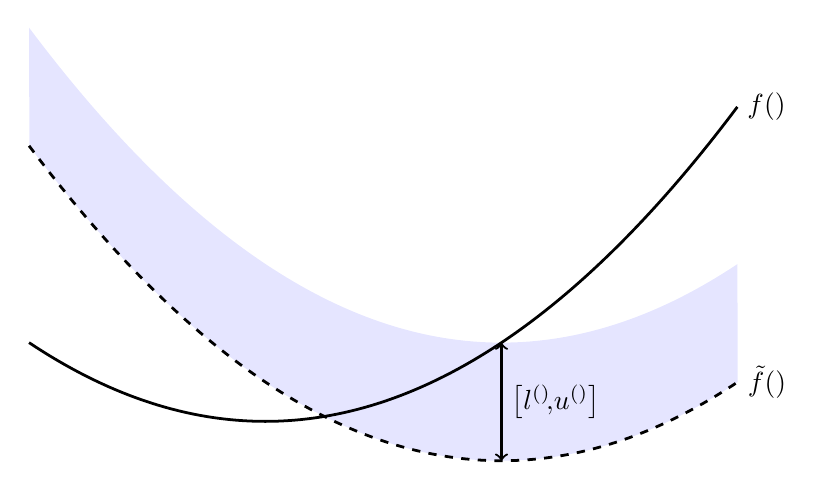
\begin{tikzpicture}[x=3cm, y=1cm]
					% Filled band around the quadratic curve with different boundary curves
					\fill[blue!10] 
					(-1, 5) -- plot[domain=-2:1, samples=100] ({\x+1}, {\x*\x + 1}) -- 
					plot[domain=1:-2, samples=100] ({\x+1}, {\x*\x - 0.5}) -- cycle;
					\node[anchor=west] at (2, 4) {$f(\weights)$};
					\draw[line width=1, domain=-2:1, samples=100,dashed] plot  ({\x+1}, {\x*\x -0.5}) node[right] {$\tilde{f}(\weights)$};
					\draw[line width=1, domain=-1:2, samples=100] plot ({\x}, {\x*\x});
					\draw[<->, thick] (1, -0.5) -- (1, 1) node[midway, right] {$\big[ l^{(\weights)}\!,\!u^{(\weights)} \big]$};
				\end{tikzpicture}
				\caption{Wir verwenden eine Schätzung $f(\weights)$ für das Leistungsmaß $\bar{f}(\weights)$ 
					um ein Konfidenzintervall $\big[ l^{(\weights)},  u^{(\weights)} \big]$ zu konstruieren. Ein Optimist 
					im Angesicht der Unsicherheit wählt Modellparameter $\weights$ gemäß dem günstigsten –
					 aber dennoch plausiblen – Wert $\tilde{f}(\weights) \defeq l^{(\weights)}$.} 
			\end{center}
	\end{figure}},first={Optimismus im Angesicht der Unsicherheit},text={Optimismus im Angesicht der Unsicherheit} 

	\newglossaryentry{minimum}
{name=Minimum,
 description={Bei einer gegebenen Menge and reeller Zahlen, ist das Minimum \index{minimum} das kleinste dieser Zahlen.},
 first={Minimum},text={Minimum}, plural={Minima}
}

\newglossaryentry{epigraph}
{name={Epigraphh},
  description={Der Epigraph \index{epigraph} einer reelwertigen Funktion $f : \mathbb{R}^n \to \mathbb{R} \cup \{+\infty\}$ 
  	is die Menge aller Punkte, die auf oder über diesem Graph liegen:
		\[
		\operatorname{epi}(f) = \left\{ (\mathbf{x}, t) \in \mathbb{R}^n \times \mathbb{R} \,\middle|\, f(\mathbf{x}) \leq t \right\}.
		\]
		Eine Funktion ist \gls{convex} genau dann, wenn ihr Epigraph eine \gls{convex}e Menge is \cite{BoydConvexBook,BertCvxAnalOpt}.
		\begin{figure}[H]
			\centering
			\begin{tikzpicture}[scale=1.0]
				\begin{axis}[
					axis lines = middle,
					xlabel = $x$,
					ylabel = {$$},
					xmin=-2, xmax=2,
					ymin=0, ymax=4.5,
					samples=100,
					domain=-1.5:1.5,
					thick,
					width=8cm,
					height=6cm,
					grid=none,
					axis on top,
					]
					% Function
					\addplot [blue, thick, domain=-1.5:1.5] {x^2} node [pos=0.85, anchor=south west, xshift=5pt] {$f(x)$};
					% Epigraph shading
					\addplot [
					name path=f,
					draw=none,
					ytick=\empty,
					domain=-1.5:1.5,
					] {x^2};
					\path[name path=top] (axis cs:-1.5,4) -- (axis cs:1.5,4);
					\addplot [
					blue!20,
					opacity=0.6,
					draw=none,
					] fill between [
					of=f and top,
					soft clip={domain=-1.5:1.5},
					];
					    \node[font=\small] at (axis cs:-1.0,2.3) {$\operatorname{epi} f$};
				%	\node[align=center, fill=white, draw=black, rounded corners, font=\small] at (axis cs:0.5,3.5) {Epigraph\\$\{(x,t) \mid f(x) \le t\}$};
				\end{axis}
			\end{tikzpicture}
			\caption{Epigraph of the function $f(x) = x^2$ (shaded area).}
		\end{figure}
	},
	first={Epigraph},
	text={Epigraph},
	plural={Epigraphen}
}


\newglossaryentry{Maximum}
{name=Maximum,
 %description={Given a set of real numbers, the maximum\index{maximum} is the largest of those numbers.},
     description={Das Maximum \index{maximum} einer Menge $\mathcal{A} \subseteq \mathbb{R}$ 
     	von reellen Zahlen ist das größte Element dieser Menge, dalls ein solches Element existiert. Eine Menge $\mathcal{A}$ 
     	besitzt ein Maximum, wenn sie nach oben beschränkt ist und ihr \gls{supremum} erreicht. \cite[Sec.~1.4]{RudinBookPrinciplesMatheAnalysis}.},
 first={Maximum},text={Maximum}, plural={Maxima}
}

\newglossaryentry{supremum}
{name=Supremum (oder kleinste obere Schranke),
	description={Das Supremum \index{supremum (oder die kleinste obere Schranke} einer Menge reeller Zahlen ist die kleinste Zahl, die größer oder gleich jedem Element der Menge ist.
	Genauer gesagt, eine reelle Zahl $a$ ist das Supremum einer Menge $\mathcal{A} \subseteq \mathbb{R}$, wenn folgende Bedingungen erfüllt sind 1) $a$ ist eine obere Schranke von $\mathcal{A}$; und 
	 2) es gibt keine Zahl die kleiner ist als $a$ und gleichzeiting ebenfalls eine obere Schranke von $\mathcal{A}$ ist. Jede nichtleere, nach oben beschränkte Menge reeller Zahlen besitzt ein Supremum, 
	 selbst dann wenn das Supremum nicht zur Menge gehört \cite[Sec.~1.4]{RudinBookPrinciplesMatheAnalysis}.},
	first={Supremum (oder kleinste obere Schranke)},text={Supremum}, plural= {Suprema}
	
    Formaler ausgedrückt ist eine reelle Zahl $a$ das Supremum einer Menge 
$\mathcal{A} \subseteq \mathbb{R}$, wenn gilt: 1) $a$ ist eine obere Schranke von $\mathcal{A}$; 
und 2) keine Zahl, die kleiner als $a$ ist, ist eine obere Schranke von $\mathcal{A}$. 
Jede nichtleere, nach oben beschränkte Menge reeller Zahlen besitzt ein Supremum, 
selbst wenn dieses Supremum nicht als Element in der Menge enthalten ist 
\cite[Abschnitt~1.4]{RudinBookPrinciplesMatheAnalysis}.
},
first={Supremum (oder kleinste obere Schranke)},
text={Supremum}
}
%potenzielle Quelle fuer Maximum und Supremum, onlinelexikon uni stuttgart : https://mo.mathematik.uni-stuttgart.de/inhalt/aussage/aussage376/
%tbc

\newglossaryentry{discrepancy}
{name=Diskrepanz,
	description={
		Consider\index{discrepancy} an \gls{fl} application with \gls{netdata} 
		represented by an \gls{empgraph}. \gls{fl} methods use a discrepancy measure 
		to compare \gls{hypothesis} maps from \gls{localmodel}s at nodes $\nodeidx,\nodeidx'$ 
		connected by an edge in the \gls{empgraph}.},
	first={discrepancy},text={discrepancy}
}

\newglossaryentry{FedRelax}
{name={FedRelax},
	description={An\index{FedRelax} \gls{fl} \gls{distributedalgorithm}. 
		\\ 
		See also: \gls{fl}, \gls{algorithm}.},
	first={FedRelax},text={FedRelax}
} 

\newglossaryentry{FedAvg}
{name={FedAvg},
	description={An\index{FedAvg} \gls{fl} \gls{algorithm} using a server-client 
		setting. 
		\\ 
		See also: \gls{fl}, \gls{algorithm}.},
	first={FedAvg},text={FedAvg}
} 

\newglossaryentry{FedGD}
{name={FedGD},
	description={An\index{FedGD} \gls{fl} \gls{distributedalgorithm} that 
		can be implemented as message passing across an \gls{empgraph}. 
		\\ 
		See also: \gls{fl}, \gls{algorithm}, \gls{gradstep}, \gls{gdmethods}.},
	first={FedGD},text={FedGD}
} 

\newglossaryentry{FedSGD}
{name={FedSGD},
	description={An\index{FedSGD} \gls{fl} \gls{distributedalgorithm} that 
		can be implemented as message passing across an \gls{empgraph}. 
		\\ 
		See also: \gls{fl}, \gls{algorithm}, \gls{gradstep}, \gls{gdmethods}, \gls{stochGD}.},
	first={FedSGD},text={FedSGD}

\newglossaryentry{hfl}
{name={horizontales kollaboratives Lernen (HFL)},description=
	{HFL\index{horizontal federated learning (HFL)} nutzt \glspl{localdataset} die aus verschiedenen
		\gls{datapoint}en, jedoch mit denselben \gls{feature}en beschrieben werden \cite{HFLChapter2020}.
	Ein Beispiel dafür ist die Wettervorhersage mit einem Netzwerk räumlich verteilter 
	Wetterbeobachtungsstationen. Jede Wetterstation misst dieselben Größen, 
	z. B. tägliche Temperatur, Luftdruck und Niederschlag.
		Allerdings erfassen die verschiedenen Stationen die Merkmale unterschiedlicher 
	raum-zeitlicher Regionen.
	Jede dieser Regionen stellt einen individuellen  \gls{datapoint}  dar, 
	der durch dieselben \glspl{feature}  (z.B. tägliche Temperatur oder Luftdruck) charakterisiert werden. \\
	Siehe auch: \gls{fl}, \gls{vfl}, \gls{cfl}. },
	first={HFL},text={HFL}
}

\newglossaryentry{dimred}
{name={Dimensionalitätsreduktion},
	description= Dimensionalitätsreduktion \index{dimensionality reduction} bezeichnet Methoden, die 
	(typischerweise viele) rohe  \glspl{feature} auf eine (relativ kleiner Menge)  neuer  \glspl{feature} abbilden.
	Diese Methoden können genutzt werden um \glspl{datapoint} zu visualisieren, indem zwei  \glspl{feature}
	gelernt weden, die als Koordinaten für die Darstellung in einem \gls{scatterplot} dienen. },
	 first={Dimensionalitätsreduktion},text={Dimensionalitätsreduktion}, plural={Dimensionalitätsreduktionen}
} 


\newglossaryentry{ml}
{name={Maschinelles Lernen (ML)},
	description={ML\index{machine learning (ML)} zielt darauf ab, ein  \gls{label} anhand der \glspl{feature} eines
		\gls{datapoint} es vorherzusagen. 
		ML-Methoden erreichen dies, indem sie eine \gls{hypothesis aus einem \gls{hypospace} (oder  \gls{model})
			durch Minimierung einer \gls{lossfunc}\cite{MLBasics},  \cite{HastieWainwrightBook} erlernen.
			Eine präzise Formulierung dieses Prinzips ist die \gls{erm}.Verschieden ML-Methoden ergeben sich aus verschiedenen 
			Designentscheidungen für \glspl{datapoint}  {d.h. deren \glspl{features und \glspl{label} }, 
				das \gls{model} und die \gls{lossfunc} \cite[Ch. 3]{MLBasics}.},
	first={Maschinelles Lernen (ML)},text={ML}
} 

\newglossaryentry{featlearn}
{name={Merkmalslernen},
	description={Betrachten wir eine  \gls{ml} Anwendung mit  \glspl{datapoint} die durch rohe  \glspl{feature} $\featurevec \in \featurespace$ beschrieben 
		werden. \Gls{feature}lernen \index{feature learning} bezeichnet die Aufgabe, eine Abbildung
		$$\featuremapvec: \featurespace \rightarrow \featurespace': \featurevec \mapsto \featurevec'$$ 
		zu lernen, welche rohe \glspl{feature} $\featurevec \in \featurespace$ eines \gls{datapoint}es einliest 
		und neue \glspl{feature} $\featurevec' \in \featurespace'$ aus einem neuen \gls{featurespace} 
		$\featurespace'$ erzeugt. Verschiedene Methoden des \gls{feature}slernens ergeben sich aus unterschiedlichen 
		Gestaltungsentscheidungen für $\featurespace,\featurespace'$,  einem \gls{hypospace} $\hypospace$ möglicher Abbildungen $\featuremapvec$
		sowie einem quantitativen Maß für die Nützlichkeit einer bestimmten Abbildung  $\featuremapvec \in \hypospace$.
		Ein Beispiel ist \gls{pca}, wobei gilt: 
		$\featurespace \defeq \mathbb{R}^{\dimlocalmodel}$, $\featurespace' \defeq \mathbb{R}^{\dimlocalmodel'}$ 
		mit $\dimlocalmodel' < \dimlocalmodel$, und ein \gls{hypospace}
		$$\hypospace\defeq \big\{ \featuremapvec: \mathbb{R}^{\dimlocalmodel}
		\!\rightarrow\! \mathbb{R}^{\dimlocalmodel'}\!:\!\featurevec'\!\defeq\!\mF \featurevec \mbox{ mit } \mF \!\in\! \mathbb{R}^{\dimlocalmodel' \times \dimlocalmodel} \big\}.$$
		\Gls{pca} bewertet die Nützlichkeit einer bestimmten Abbildung $\featuremapvec(\featurevec)= \mF \featurevec$ 
		durch den \gls{minimalen} linearen Rekonstruktionsfehler auf einem \gls{dataset}, also
		$$ \min_{\mG \in \mathbb{R}^{\dimlocalmodel \times \dimlocalmodel'}} \sum_{\sampleidx=1}^{\samplesize} \normgeneric{\mG \mF \
	first={Merkmalslernen},text={Merkmalslernen}
} 


\newglossaryentry{autoencoder}
{name={Autokodierer},
	description={Ein Autokodierer r\index{Autoencoder} ist eine \gls{ml}- Methode, die gleichzeitig ein Kodierer-Abbildung 
		$\hypothesis(\cdot) \in \hypospace$  und eine dekodierer Abbildung  $\hypothesis^{*}(\cdot) \in \hypospace^{*}$ erlernt. 
		Dies ist ein Beispiel für \gls{erm}, bei dem der \gls{erm}  aus dem Rekonstruktionsfehler, $\featurevec - \hypothesis^{*}\big(  \hypothesis \big( \featurevec \big) \big)$. berechnet wird},
	first={Autokodierer},text={Autokodierer}
} 

\newglossaryentry{vfl}
{name={Vertikales Kollaboratives Lernen (VFL)},
	description={
		VFL\index{vertical federated learning (VFL)} beschreibt  \gls{fl}  Anwendungen bei denen 
		\gls{device}s Zugang zu verschiedenen  \gls{feature}s desselben  \gls{datapoint}es  \cite{VFLChapter} haben. 
		Das zugrunde liegende globale \gls{dataset ist 
		\[
		\dataset^{(\mathrm{global})} \defeq \left\{ \left(\featurevec^{(1)}, \truelabel^{(1)}\right), \ldots, \left(\featurevec^{(\samplesize)}, \truelabel^{(\samplesize)}\right) \right\}.
		\]
		Wir kennzeichnen  $\featurevec^{(\sampleidx)} = \big( \feature^{(\sampleidx)}_{1}, \ldots, \feature^{(\sampleidx)}_{\nrfeatures'} \big)^{T}$, für $\sampleidx=1,\ldots,\samplesize$, 
		als den kompletten  \gls{featurevec}s für die \glspl{datapoint} . Jedes \gls{device} $\nodeidx \in \nodes$ 
		hat Zugang zu nur einem Teilset  $\mathcal{F}^{(\nodeidx)} \subseteq \{1,\ldots,\nrfeatures'\}$ von  \glspl{feature}s, aus dem ein  
		 \gls{localdataset}  $\localdataset{\nodeidx}$ resultiert mit  \glspl{featurevec}
		\[
		\featurevec^{(\nodeidx,\sampleidx)} = \big( \feature^{(\sampleidx)}_{\featureidx_{1}}, \ldots, \feature^{(\sampleidx)}_{\featureidx_{\nrfeatures}} \big)^{T}.
		\]
		Einige  \glspl{device} können auch Zugang zu den \glspl{label} $\truelabel^{(\sampleidx)}$, for $\sampleidx=1,\ldots,\samplesize$, des globalen \gls{dataset}s haben. Eine potentielle Anwendung für \gls{vfl} sind Kollaborationen zwischen verschiedenen Gesundheitsdienstleistern. 
		Jeder Dienstleister sammelt bestimmte Messungen wie Blutwerte, Elektrokardiographien und Röntgenaufnahmen der Lunge für den selben Patienten. 
		Einer weitere Anwendung ist ein nationales Sozialversicherungssystem, in dem Gesundheitsdaten, finanzielle Indikatoren, Verbraucherverhalten und Mobilitäts\glspl{data} von verschiedenen Institutionen gesammelt werden.  \gls{vfl} ermöglicht gemeinsames lernen zwischen diesen Parteien und gleichzeitig ein genau definiertes Maß an \gls{privprot}.
		
		\begin{figure}[htbp]
			\begin{center}
				\begin{tikzpicture}[every node/.style={anchor=base}]
					% --- Coordinate definitions ---
					\def\colX{0}
					\def\colY{1.6}
					\def\colZ{3.2}
					\def\colD{4.8}
					\def\colLabel{6.4} 
					\def\rowOne{0}
					\def\rowTwo{-1.2}
					\def\rowThree{-2.4}
					\def\rowFour{-3.6}
					% Manually place matrix entries
					\foreach \i/\label in {1/1, 2/2, 4/\samplesize} {
						\pgfmathsetmacro{\y}{-1.2*(\i-1)}
						\node (x\i1) at (0,\y) {$x^{(\label)}_{1}$};
						\node (x\i2) at (1.6,\y) {$x^{(\label)}_{2}$};
						\node (dots\i) at (3.2,\y) {$\cdots$};
						\node (x\i3) at (4.8,\y) {$x^{(\label)}_{\dimlocalmodel}$};
						\node (y\i) at (6.4,\y) {$\truelabel^{(\label)}$};
					}
					% Outer rectangle for the full dataset
					\draw[dashed, rounded corners, thick]
					(-0.6,0.6) rectangle (6.9,-4.2);
					\node at (3.1,0.9) {$\dataset^{(\mathrm{global})} $};
					% Rectangle for local dataset 1 (e.g., first two features)
					\draw[dashed, rounded corners, thick]
					(-0.9,0.9) rectangle (2.1,-4.0);
					\node at (0.25,1.0) {$\localdataset{1}$};
					% --- Local dataset k (columns 2–3, rows 1–3) ---
					\draw[dashed, rounded corners, thick]
					($( \colZ + 1,,0.9 )$) rectangle
					($( \colLabel + 0.4, -4.5)$);
					\node at ($( \colZ + 0.9,-5 )$) {$\localdataset{\nodeidx}$};
				\end{tikzpicture}
			\end{center}
			\caption{VFL nutzt \glspl{localdataset}  die von  \glspl{datapoint} eines gemeinsamen globalen \gls{dataset}es abgeleitet sind. 
				Die \glspl{localdataset} unterschieden sich in der Wahl der \glspl{feature} die verwendet werden, um die  \glspl{datapoint} zu charakterisieren.
				\label{fig_vertical_FL}}
	\end{figure}},
	first={Vertikales Kollaboratives Lernen (VFL)},text={VFL}
} 

\newglossaryentry{interpretability}
{name={Interpretierbarkeit},description=
	{Eine \gls{ml} -Methode  ist interpretierbar \index{interpretability} für einen bestimmten Nutzer, wenn er die 
	 \glspl{prediction}, die von der Methode geliefert werden, gut vorhersehen kann. Der Begriff der Interpretierbarkeit 
	 lässt sich  durch quantitative Maße der  \gls{uncertainty} über die \gls{prediction}s präzisieren \cite{JunXML2020}.},
	first={Interpretierbarkeit},text={Interpretierbarkeit}
}

\newglossaryentry{multitask learning}
{name={Multitask Lernen },description=
	{Multitask Lernen \index{multitask learning} zielt darauf ab, Beziehungen  zwischen verschiedenen  \glspl{learningtask} auszunutzen.
	Betrachten wir zwei  \glspl{learningtask} die vom gleichen  \gls{dataset} bestehend aus webcam Bildaufnahmen, gewonnen werden. 
	Die erste  \gls{learningtask} besteht darin, die Anwesenheit eines Menschen zu bestimmen, die zweite Aufgabe hingegen ist die Anwesenheit 
	eines Autos zu bestimmen. Es kann sinnvol sein, die gleiche  \gls{deepnet} Struktur für beide  \glspl{learningtask}  zu verwenden und nur die \gls{weights} 
	der finalen Ausgabeschicht unterschiedlich zu gestalten. 
	
		 Consider two \gls{learningtask}s obtained from the  \gls{deepnet} 
		same \gls{dataset} of webcam snapshots. The first task is to predict the presence 
		of a human, while the second task is to predict the presence of a car. It might be useful 
		to use the same \gls{deepnet} structure for both tasks and only allow the \gls{weights} of 
		the final output layer to be different.},
	first={Multitask Lernen},text={Multitask Lernen}
}

\newglossaryentry{learningtask}
{name={Lernaufgabe},description=
	{Consider\index{learning task} a \gls{dataset} $\dataset$ constituted by several \gls{datapoint}s, each of them 
		characterized by \gls{feature}s $\featurevec$. For example, the \gls{dataset} $\dataset$ 
		might be constituted by the images of a particular database. Sometimes it might be useful 
		to represent a \gls{dataset} $\dataset$, along with the choice of \gls{feature}s, by a \gls{probdist} $p(\featurevec)$. 
		A learning task associated with $\dataset$ consists of a specific 
		choice for the \gls{label} of a \gls{datapoint} and the corresponding \gls{labelspace}. 
		Given a choice for the \gls{lossfunc} and \gls{model}, a learning task gives rise to an 
		instance of \gls{erm}. Thus, we could define a learning task also via an instance of \gls{erm}, i.e., 
		via an \gls{objfunc}. Note that, for the same \gls{dataset}, we obtain different learning tasks by using 
		different choices for the \gls{feature}s and \gls{label} of a \gls{datapoint}. These learning 
		tasks are related, as they are based on the same \gls{dataset}, and solving them jointly 
		(via \gls{multitask learning} methods) is typically preferable over solving them separately \cite{Caruana:1997wk}, \cite{JungGaphLassoSPL}, \cite{CSGraphSelJournal}.},
	first={Lernaufgabe},text={{name={Lernaufgabe},description=
			{Betrachten wir eine \index{learning task}  mit einem  \gls{dataset} $\dataset$ bestehen aus verschiedenen  \glspl{datapoint}n, jeder charakterisiert durch  \glspl{feature}  $\featurevec$. 
				Der \gls{dataset} $\dataset$  könnte beispielsweise aus Bildern aus einer bestimmten Datenbank bestehen. 
				Manchmal kann es hier hilfreich sein, den  \gls{dataset} $\dataset$ zusammen mit der Wahl der  \glspl{feature} durch eine  \gls{probdist} $p(\featurevec)$ zu repräsentieren. 
				Eine Lernaufgabe, die mit  $\dataset$ assoziiert ist, besteht aus einer spezifischen Wahl des \gls{label}s für einen \gls{datapoint}, sowie des zugehörigen  \gls{labelspace}es. 
				Bei gegebener Wahl der  \gls{lossfunc} und des \gls{model}s, ergibt sich aus einer Lernaufgabe eine Instanz 
				von \gls{erm}. Daher kann man eine Lernaufgabe auch direkt durch eine Instanz von \gls{erm}, 
				d. h. über eine \gls{objfunc}, definieren.
				
				Beachte, dass sich aus demselben \gls{dataset} unterschiedliche Lernaufgaben ergeben, wenn man 
				unterschiedliche \gls{feature}s und \gls{label} für einen \gls{datapoint} wählt. 
				Diese Lernaufgaben sind miteinander verwandt, da sie auf demselben \gls{dataset} basieren. 
				Es ist in der Regel vorteilhaft, sie gemeinsam (z. B. durch \gls{multitask learning}-Methoden) 
				zu lösen, anstatt sie getrennt zu behandeln \cite{Caruana:1997wk}, \cite{JungGaphLassoSPL}, \cite{CSGraphSelJournal}.
				},
				first={Lernaufgabe},text={Lernaufgabe}
			}
		
		
				\newglossaryentry{explainability}
				{name={Erklärbarkeit},description=
					{Wir \index{explainability} definierien die subjektive Erklärbarkeit einer \gls{ml}- Methode als Maß für den Grad der 
						Simulierbarkeit \cite{Colin:2022aa} der von einem \gls{ml}- System gelieferten \glspl{prediction} fü einen menschlichen Nutzer. Quantiative Maße der subjektiven Erllärbarkeit eines trainierten \gls{model}s können konstruiert werden, in dem man dessen 
						\glspl{prediction} mit den \glspl{prediction} vergleicht, die von einem Nutzer durch ein \gls{testset} bereitgestellt werden \cite{Colin:2022aa}, \cite{Zhang:2024aa}. 
						Alternativ können wir 
						Alternatively, we can use \glspl{probmodel} für  \gls{data} verwednen und die Erklärbarkeit eines trainierten \gls{ml} 
						\gls{model}s über die konditionale (bzw. differentielle) Entropie seiner  \glspl{prediction}, bei gegebenen \glspl{prediction} der Nutzer messen \cite{JunXML2020}, \cite{Chen2018}. 
					},
					first={Erklärbarkeit},text={Erklärbarkeit}
				}
				
				
				\newglossaryentry{lime}
				{name={lokale interpretierbare modellunabhängige Erklärungen (LIME)},
					description={
						Betrachten wir \index{local interpretable model-agnostic explanations (LIME)} eine trainiertes  \gls{model} (oder erlernte \gls{hypothesis}) $\widehat{\hypothesis} \in \hypospace$, die den \gls{featurevec} eines  \gls{datapoint}es auf die \gls{prediction} $\widehat{\truelabel}= \widehat{\hypothesis}$ abbildet. 
						Lokale interåretierbare \gls{model}-agnostische \glspl{explanation} sind eine Technik zur Erklärung des Verhalten von $\widehat{\hypothesis}$ 
						lokal um einen \gls{datapoint} mit \gls{featurevec} $\featurevec^{(0)}$ \cite{Ribeiro2016}. 
						Diese Annäherung kann durch eine Instanz von \gls{erm} mit sorgfältig gewähltem \gls{trainset} gewonnen werden. 
						Insbesondere besteht das \gls{trainset} aus \glspl{datapoint} mit \gls{featurevec} $\featurevec$, die nahe bei 
						$\featurevec^{(0)}$ liegen und  aus dem (Pseudo-)Label $\widehat{\hypothesis}(\featurevec)$. 
						Beachte, dass für die Annäherung ein anderes \gls{model} $\hypospace'$ verwendet werden kann als für das Originalmodell $\hypospace$. 
						Zum Beispiel kann ein \gls{decisiontree} verwendet werden, um lokal ein \gls{deepnet} zu approximieren. 
						Eine weitere häufig verwendete Wahl für $\hypospace'$ ist das \gls{linmodel}.
					
						\begin{figure}[H]
							\begin{center}
								\begin{tikzpicture}
									\begin{axis}[
										axis lines=middle,
										xlabel={$\featurevec$},
										ylabel={$\truelabel$},
										xtick=\empty,
										ytick=\empty,
										xmin=0, xmax=6,
										ymin=0, ymax=6,
										domain=0:6,
										samples=100,
										width=10cm,
										height=6cm,
										clip=false
										]
										% Non-linear model h(x)
										\addplot[blue, thick, domain=0:6] {2 + sin(deg(x))} node[pos=0.85, above right,yshift=3pt] {$\widehat{\hypothesis}(\featurevec)$};
										% Feature value x0
										\addplot[dashed, gray] coordinates {(3,0) (3,6)};
										% Piecewise constant local approximation g(x)
										\addplot[red, thick, domain=2.5:3.5] {2 + sin(deg(3))} node[pos=0.9, above] {$g(\featurevec)$};
										% Optional: mark the point of approximation
										\addplot[mark=*] coordinates {(3, {2 + sin(deg(3))})};
										\node at (axis cs:3,-0.3) {$\featurevec^{(0)}$};
									\end{axis}
								\end{tikzpicture}
							\end{center}
							\caption{{Zur Erklärung eines trainierten \gls{model} $\widehat{\hypothesis} \in \hypospace$ 
									in der Umgebung eines gegebenen \gls{featurevec} $\featurevec^{(0)}$ kann eine lokale Approximation $g \in \hypospace'$ verwendet werden.}
							\label{fig_lime}
					\end{figure}},
					first={LIME},text={LIME}
				}
				
\newglossaryentry{linmodel}{name={Lineares Modell},
	description={Betrachten wir \index{linear model}  \glspl{datapoint}, die jeweils durch einen numerischen {featurevec} 
		$\featurevec \in \mathbb{R}^{\featuredim}$ charakterisiert sind . Ein lineares  \gls{model} ist 
		ein  \gls{hypospace} der aus linearen Abbildungen besteht, sodass : 
		\begin{equation} 
			\label{equ_def_lin_model_hypspace_dict}
			\linmodel{\nrfeatures} \defeq \left\{ \hypothesis(\featurevec)= \weights^{T} \featurevec: \weights \in \mathbb{R}^{\nrfeatures} \right\}. 
		\end{equation} 
		Beachte, dass  \eqref{equ_def_lin_model_hypspace_dict} eine ganze Familie von \glspl{hypospace}definiert, die 
		durch die Anzahl von $\nrfeatures$ der \gls{feature}s  parametrisiert ist , die linear kombiniert werden, um die 
		\gls{prediction} $\hypothesis(\featurevec)$  zu berechnen. 
		Die Wahl von $\nrfeatures$ wird durch \gls{compasp} (z.\,B. eine kleinere $\nrfeatures$ reduziert den Rechenaufwand), 
		\gls{statasp} (z.\,B. eine größere $\nrfeatures$ kann den \gls{prediction}fehler verringern) 
		und \gls{interpretability} beeinflusst. Ein lineares \gls{model}, das nur wenige, aber gezielt gewählte 
		\glspl{feature} nutzt, gilt typischerweise als besser interpretierbar \cite{rudin2019stop}, \cite{Ribeiro2016}.
		},
		first={lineares Modell},text={lineares Modell}
	}


\newglossaryentry{gradstep}{name={Gradientenschritt},
	description= Gegeben sei eine \gls{differentiable} reellwertiger Funktion$f(\cdot): \mathbb{R}^{\nrfeatures} \rightarrow \mathbb{R}$  und ein Vektor 
		$\weights \in \mathbb{R}^{\nrfeatures}$. Der  \gls{gradient}enschritt \index{gradient step} aktualisiert  $\weights$ indem der skalierte negative \gls{gradient} $\nabla f(\weights)$ addiert wird.(siehe Fig. \ref{fig_basic_GD_step_single_dict})
	
		\begin{equation}
			\label{equ_def_gd_basic_dict} 
			\widehat{\weights}  \defeq \weights - \lrate \nabla f(\weights).
		\end{equation} 
		 Mathematisch ist der  \gls{gradient}enschritt ein (typischerweise nichtlinearer) Operator  $\mathcal{T}^{(f,\lrate)}$ der durch die Funktion $f$
		 und die  \gls{stepsize} $\lrate$ parametrisiert wird. 
	
		\begin{figure}[H]
			\begin{center}
				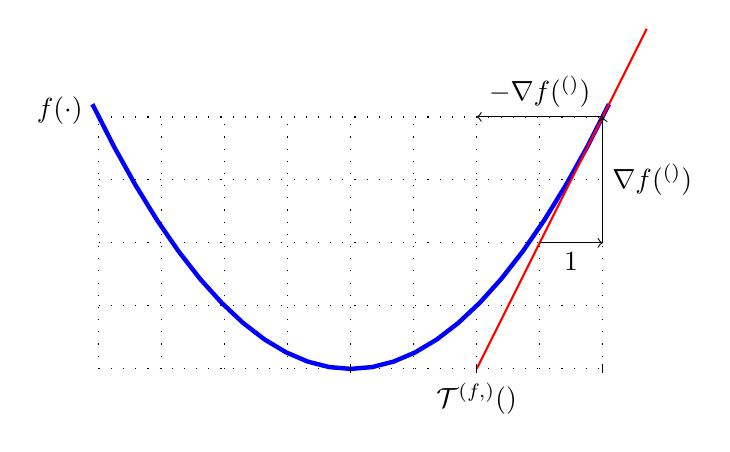
\begin{tikzpicture}[scale=0.8]
					\draw[loosely dotted] (-4,0) grid (4,4);
					\draw[blue, ultra thick, domain=-4.1:4.1] plot (\x,  {(1/4)*\x*\x});
					\draw[red, thick, domain=2:4.7] plot (\x,  {2*\x - 4});
					\draw[<-] (4,4) -- node[right] {$\nabla f(\weights^{(\itercntr)})$} (4,2);
					\draw[->] (4,4) -- node[above] {$-\lrate \nabla f(\weights^{(\itercntr)})$} (2,4);
					\draw[<-] (4,2) -- node[below] {$1$} (3,2) ;
					%\draw[->] (-4.25,0) -- (4.25,0) node[right] {$a$};
					\node[left] at (-4.1, 4.1) {$f(\cdot)$}; 
					\draw[shift={(0,0)}] (0pt,2pt) -- (0pt,-2pt) node[below] {$\overline{\weights}$};
					\draw[shift={(4,0)}] (0pt,2pt) -- (0pt,-2pt) node[below] {$\weights$};
					\draw[shift={(2,0)}] (0pt,2pt) -- (0pt,-2pt) node[below] {$\mathcal{T}^{(f,\lrate)}(\weights)$};
				\end{tikzpicture}
			\end{center}
			\caption{Der grundlegende \gls{gradient} enschjritt \eqref{equ_def_gd_basic_dict}  bildet einen gegebenen Vektro  $\weights$ 
				auf den aktualisierten Vektor $\weights'$ ab. Er definiert einen Operator,
				$\mathcal{T}^{(f,\lrate)}(\cdot): \mathbb{R}^{\nrfeatures} \rightarrow \mathbb{R}^{\nrfeatures}:
				\weights \mapsto \widehat{\weights}$.}
			\label{fig_basic_GD_step_single_dict}
		\end{figure}
		Beachte das der  \gls{gradient}enschritt \eqref{equ_def_gd_basic_dict} lokal optimisiert - in einer \gls{neighborhood}, deren Größe durch die  \gls{stepsize} $\lrate$, eine lineare Annäherung an die Funktion $f(\cdot)$ bestimmt wird.  
		Eine naheliegende  \gls{Verallgemeinerung} 
		von \eqref{equ_def_gd_basic_dict} besteht darin, die Funktion selbst, statt der linearen Annäherung,  lokal zu optimieren, sodass:
		
		\begin{align} 
			\label{equ_approx_gd_step_dict}
			\widehat{\weights} = \argmin_{\weights' \in \mathbb{R}^{\dimlocalmodel}} f(\weights')\!+\!(1/\lrate)\normgeneric{\weights-\weights'}{2}^2. 
		\end{align}
		Wir verwenden absichtlich das gleiche Symbol $\lrate$ wie in \eqref{equ_def_gd_basic_dict}, 
		da auch hier gilt: Je größer $\lrate$, desto größer typischerweise der Fortschritt hin zu 
		einem kleineren Funktionswert $f(\widehat{\weights})$. Ähnlich wie der Gradientenschritt 
		\eqref{equ_def_gd_basic_dict} definiert auch die Aktualisierung \eqref{equ_approx_gd_step_dict} 
		einen (typischerweise nichtlinearen) Operator, der durch die Funktion $f(\cdot)$ und den Parameter 
		$\lrate$ bestimmt ist. Für eine \gls{konvexe} Funktion $f(\cdot)$ ist dieser Operator auch als 
		\gls{proxop} der Funktion bekannt \cite{ProximalMethods}.
		},
		first={Gradientenschritt},text={Gradientenschritt},plural={Gradientenschritte}
}

\newglossaryentry{proxop}
{name={Proximaloperator},
	description={Gegeben sei \index{proximal operator} eine \gls{convex}e Funktion $f(\weights')$. Wir definieren ihren Proximal Operator gemäß \cite{ProximalMethods}, \cite{Bauschke:2017} als: 
		$$\proximityop{f(\cdot)}{\weights}{\rho}\defeq \argmin_{\weights' \in \mathbb{R}^{\dimlocalmodel}} \bigg[ f(\weights')\!+\!(\rho/2) \normgeneric{\weights- \weights'}{2}^{2}\bigg] \mbox{ mit } \rho > 0. $$ 
		Wie in Fig. \ref{fig_proxoperator_opt_dict}  illustriert, entspricht die Auswertung des Proximaloperators der Minimierung einer penalisierten Variante von $f(\weights')$. Der Strafterm ist der skalierte quadratische euklidische Abstand zu einem gegebenen Vektor $\weights$ (welcher der Eingabewert des Proximaloperators ist).
	
		%\Gls{convex} functions for which the proximal operator can be computed efficiently 
		%is sometimes referred to as \emph{proximable} or \emph{simple} \cite{Condat2013}. 
		Der Proximaloperator kann als eine \gls{generalization} des e \gls{gradstep}s interpretiert werden, der für eine \gls{smooth} \gls{convex}e Funktion  $f(\weights') $ definiert ist. Tatsächlich entspricht ein
		\gls{gradstep} mit \gls{stepsize} $\lrate$ am momentanen Vektor r $\weights$ der Anwendung des Proximaloperators der Funktion 
		 $\tilde{f}(\weights')= \big( \nabla f(\weights)\big)^{T} (\weights'-\weights)$ 
		mit $\rho=1/\lrate$.
		\begin{figure}[H]
			\begin{center}
				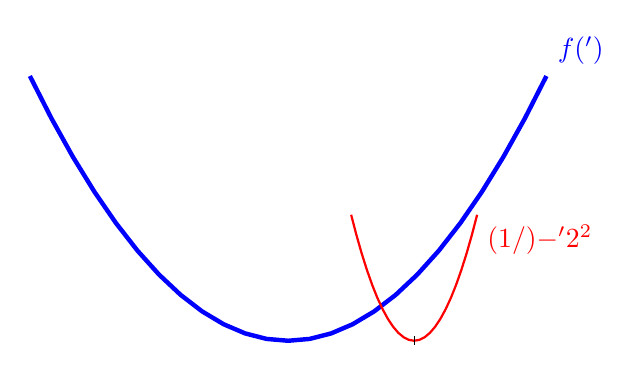
\begin{tikzpicture}[scale=0.8]
					% Original quadratic function
					\draw[blue, ultra thick, domain=-4.1:4.1] plot (\x, {(1/4)*\x*\x}) node[above right] {$f(\weights')$};		
					% Quadratic function with larger curvature, centered at w = 2
					\draw[red, thick, domain=1:3] plot (\x, {2*(\x - 2)*(\x - 2)}) node[below right] {$(1/\lrate)\normgeneric{\weights-\weights'}{2}^{2}$};
					% Axes
					% Minimum point of second curve
					\draw[shift={(2,0)}] (0pt,2pt) -- (0pt,-2pt) node[below] {$\weights$};
					%\node at (2,0.5) [anchor=north] {$\weights$};
				\end{tikzpicture}
			\end{center}
			\caption{A generalized \gls{gradstep} updates a vector $\weights$ by minimizing a penalized version 
				of the function $f(\cdot)$. The penalty term is the scaled squared Euclidean distance between the optimization 
				variable $\weights'$ and the given vector $\weights$.	\label{fig_proxoperator_opt_dict}}
		\end{figure}
	},first={proximal operator},text={proximal operator}}
}

	
	\newglossaryentry{proximable}
	{name={proximable},
		description={Eine \index{proximable} 
			\gls{convex}e Funktion für die der  \gls{proxop} effizient berechnet werden kann, wird manchmal als proximierbar oder 
			einfach bezeichnet  \cite{Condat2013}.},
			first={proximable},text={proximable}, plural={proximablen}
			
			
			}

\newglossaryentry{connected}
{name ={zusammenhängender Graph}, 
	description={Ein \index{connected graph} ungerichteter \gls{graph} $\graph=\pair{\nodes}{\edges}$ 
		heißt zusammenhängend \index{connected graph}  wenn jede nicht-leere Teilmenge  $\nodes' \subset \nodes$ 
		zumindest eine Kante besitzt, die $\nodes$ mit $\nodes \setminus \nodes'$ verbindet.}, 
	first={zusammenhängender Graph},text={zusammenhängender Graph}, plural={zusammenhängende Graphen}
	
	}

\newglossaryentry{mvndist}
{name ={multivariate Normalverteilung}, 
	description={Die \index{multivariate normal distribution} multivariate Normalverteilung
		$\mvnormal{\vm}{\mC}$ ist eine wichtige Familie von \gls{probdist}s  für eine stetige  \gls{rv} $\featurevec \in \mathbb{R}^{\nrfeatures}$ \cite{BertsekasProb}, \cite{GrayProbBook}, \cite{Lapidoth09}. 
		Diese Familie is parametrisiert durch den \gls{mean} $\vm$  und die  \gls{covmtx} $\mC$ von $\featurevec$. 
		If the \gls{covmtx} is invertible, the \gls{probdist} of $\featurevec$ is 
		$$p(\featurevec) \propto \exp\bigg(-(1/2) \big( \featurevec - \vm \big)^{T} \mC^{-1} \big( \featurevec - \vm \big) \bigg).$$},
		 first={Multivariate Normalverteilung},text={multivariate Normalverteilung}}
		 
		 
 \newglossaryentry{statasp}
		 {name ={statistische Aspekte}, 
		 	description={Unter statistischen Aspekten\index{statistical aspects} einer  \gls{ml}-Methode versteht man (Eigenschaften) der \gls{probdist}
		 		seiner Ausgabe unter einem a \gls{probmodel} für die  \gls{data}, die in das Verfahren eingespeisst werden.},
		 		first={Statistische Aspekte},text={statistische Aspekte}}

\newglossaryentry{compasp}
{name={rechnerische Aspekte},
	description={Unter rechnerischen Aspekten \index{computational aspects} eines \gls{ml}-Verfahrens verstehen wir hauptsächlich die für dessen Implementierung erforderlichen Rechenressourcen. Zum Beispiel umfasst bei einem \gls{ml}-Verfahren, das iterative Optimierungstechniken zur Lösung von \gls{erm} verwendet, die computational aspects: 1) wie viele arithmetische Operationen für eine einzelne Iteration (d.h. einen \gls{gradstep}) benötigt werden; und 2) wie viele Iterationen erforderlich sind, um nützliche \gls{modelparams} zu erhalten. Ein wichtiges Beispiel für eine iterative Optimierungstechnik ist \gls{gd}.},
	first={Rechnerische Aspekte},
	text={rechnerische Aspekte}
}

\newglossaryentry{zerooneloss}
{name={$\bf 0/1$ Verlust},
	description={Der $0/1$ \gls{loss}\index{$0/1$ loss} $\lossfunczo{\pair{\featurevec}{\truelabel}}{\hypothesis}$ misst die Qualität eines \gls{classifier} $\hypothesis(\featurevec)$, der eine \gls{prediction} $\predictedlabel$ liefert (z. B. durch Thresholding \eqref{equ_def_threshold_bin_classifier_dict}) für das \gls{label} $\truelabel$ eines \gls{datapoint} mit \gls{feature}s $\featurevec$. Er ist gleich $0$, wenn die \gls{prediction} korrekt ist, d.h. $\lossfunczo{\pair{\featurevec}{\truelabel}}{\hypothesis}=0$, wenn $\predictedlabel=\truelabel$. Er ist gleich $1$, wenn die \gls{prediction} falsch ist, d.h. $\lossfunczo{\pair{\featurevec}{\truelabel}}{\hypothesis}=1$, wenn $\predictedlabel \neq \truelabel$.},
	sort=zerooneloss,
	first={$0/1$ Verlust},
	text={$0/1$ Verlust}
}


\newglossaryentry{probability}
{name={Wahrscheinlichkeit},
	description={Wir\index{probability} ordnen jedem Ereignis, das bei einem Zufallsexperiment auftreten kann, einen Wahrscheinlichkeitswert zu, der typischerweise im Intervall $[0,1]$ liegt \cite{BertsekasProb}, \cite{HalmosMeasure}, \cite{BillingsleyProbMeasure}, \cite{KallenbergBook}.},
	first={Wahrscheinlichkeit},
	text={Wahrscheinlichkeit}
	plural={Wahrscheinlichkeiten}
}

\newglossaryentry{underfitting}
{name={Unteranpassung},
	description={Betrachten wir eine \gls{ml}-Methode, die \gls{erm} verwendet, um eine \gls{hypothesis} mit dem minimalen \gls{emprisk} auf einem gegebenen \gls{trainset} zu lernen. Eine solche Methode unterfitttet das \gls{trainset}, wenn sie nicht in der Lage ist, eine \gls{hypothesis} mit ausreichend kleinem \gls{emprisk} auf dem \gls{trainset} zu lernen. Wenn eine Methode Unteranpassung aufweist, ist sie typischerweise auch nicht in der Lage, eine \gls{hypothesis} mit kleinem \gls{risk} zu lernen.},
	first={Unteranpassung},
	text={Unteranpassung}
}


\newglossaryentry{overfitting}
{name={Überanpassung}},
	description={Betrachten wir eine \gls{ml}-Methode, die \gls{erm} verwendet, um eine \gls{hypothesis} mit dem minimalen \gls{emprisk} auf einem gegebenen \gls{trainset} zu lernen. Eine solche Methode ist überangepasst an das \gls{trainset}, wenn sie eine \gls{hypothesis} mit kleinem \gls{emprisk} auf dem \gls{trainset} lernt, aber außerhalb des \gls{trainset} einen deutlich größeren \gls{loss} aufweist.},
	first={Überanpassung},
	text=Überanpassung}
}

\newglossaryentry{gdpr}{name={ Datenschutz-Grundverordnung (DSGVO)},description={
		Die The\index{general data protection regulation (GDPR)} DGSVO
		urde von der Europäischen Union (EU) erlassen und ist seit dem 25. Mai 2018 wirksam \cite{GDPR2016}. 
		 Sie schützt die Privatsphäre und die \gls{data}-Rechte von Personen in der EU. Die DGSVO hat weitreichende Auswirkungen darauf, wie \gls{data} in \gls{ml}-Anwendungen gesammelt, gespeichert und genutzt werden. Wichtige Bestimmungen umfassen:
		\begin{itemize}
			 \item \Gls{dataminprinc}: \gls{ml}-Systeme sollten nur die notwendige Menge an persönlichen \gls{data} für ihren Zweck verwenden.
			\item \Gls{transparency} und \gls{explainability}: \gls{ml}-Systeme sollten ihren Nutzern ermöglichen, zu verstehen, wie Entscheidungen getroffen werden, die die Nutzer betreffen.
			\item Rechte der Betroffenen: Nutzer sollten die Möglichkeit erhalten, auf ihre persönlichen \gls{data} zuzugreifen, diese zu berichtigen und zu löschen sowie der automatisierten Entscheidungsfindung und Profilbildung zu widersprechen.
			\item Verantwortlichkeit: Organisationen müssen eine robuste \gls{data}-Sicherheit gewährleisten und die Einhaltung durch Dokumentation und regelmäßige Audits nachweisen.
		\end{itemize}
	}, 
	first={ Datenschutz-Grundverordnung (DSGVO)},text={DSGVO}
	
\newglossaryentry{gaussrv}{
	name={Gaußsche Zufallsvariable (Gaußsche ZV)},
	description={
		Eine \index{Gaußsche Zufallsvariable (Gaußsche ZV)} standard-Gaußsche \gls{rv} ist eine 
		reellwertige \gls{rv} $x$ mit der \gls{pdf} \cite{BertsekasProb}, \cite{GrayProbBook}, \cite{papoulis}
		\begin{equation}
			\nonumber
			p(x) = \frac{1}{\sqrt{2\pi}} \exp^{-x^2/2}.
		\end{equation}
		Ausgehend von einer standard-Gaußschen \gls{rv} $x$ lässt sich eine allgemeine Gaußsche \gls{rv} $x'$ 
		mit \gls{mean} $\mu$ und \gls{variance} $\sigma^2$ durch $x' \defeq \sigma (x + \mu)$ konstruieren. 
		Die \gls{probdist} einer Gaußschen \gls{rv} wird als Normalverteilung bezeichnet und mit 
		$\mathcal{N}(\mu, \sigma)$ notiert. \\ 
		Ein Gaußscher Zufallsvektor $\featurevec \in \mathbb{R}^{\featuredim}$ mit 
		\gls{covmtx} $\mathbf{C}$ und \gls{mean} ${\bm \mu}$ kann durch 
		$\featurevec \defeq \mathbf{A} \big( \vz + {\bm \mu} \big)$ erzeugt werden. 
		Dabei ist $\mA$ eine Matrix, die $\mA\mA^{T} = \mC$ erfüllt, 
		und $\vz \defeq \big( z_{1},\ldots,z_{\featuredim} \big)^{T}$ ist ein Vektor, dessen Einträge 
		\gls{iid} standard-Gaußsche \gls{rv}s $z_{1},\ldots,z_{\featuredim}$ sind. \\
		Gaußsche Zufallsvektoren sind ein Spezialfall von Gaußschen Prozessen, 
		die als lineare Transformationen unendlicher Folgen von standard-Gaußschen \gls{rv}s 
		aufgefasst werden können \cite{Rasmussen2006Gaussian}. \\
		Gaußsche \gls{rv}s sind weit verbreitete \gls{probmodel}s in der statistischen Analyse 
		von \gls{ml}-Methoden. Ihre Bedeutung ergibt sich unter anderem aus dem zentralen Grenzwertsatz, 
		welcher besagt, dass der Mittelwert einer wachsenden Anzahl unabhängiger \gls{rv}s 
		(die selbst nicht notwendigerweise gaußverteilt sind) gegen eine Gaußsche \gls{rv} konvergiert 
		\cite{ross2013first}. \\
		Siehe auch: \gls{probdist}, \gls{probdist}, \gls{probspace}.
	},
	first={Gaußsche Zufallsvariable (Gaußsche ZV)},
	text={Gaußsche ZV}
}
	
\newglossaryentry{GaussProc}
{name={Gauß-Prozess (GP)},
	description={Ein \index{Gauß-Prozess (GP)}Gauß-Prozess ist eine Familie von \gls{rv}s 
		$\{f(\featurevec)\}_{\featurevec \in \featurespace}$, die durch Eingabewerte $\featurevec$ 
		aus einem Eingaberaum $\featurespace$ indiziert sind. Für jede endliche Teilmenge 
		$\featurevec^{(1)}, \ldots, \featurevec^{(\samplesize)} \in \featurespace$ 
		haben die entsprechenden \gls{rv}s $f(\featurevec^{(1)}), \ldots, f(\featurevec^{(\samplesize)})$ 
		eine gemeinsame multivariate Normalverteilung:
		\[
		\left( f(\featurevec^{(1)}), \ldots, f(\featurevec^{(\samplesize)}) \right) \sim \mathcal{N}(\boldsymbol{\mu}, \mathbf{K}).
		\]
		Für einen festen Eingaberaum $\featurespace$ ist ein Gauß-Prozess vollständig definiert durch:
		\begin{itemize}
			\item eine \gls{mean}-Funktion $\mu(\featurevec) = \expect\{ f(\featurevec)\}$,
			\item und eine Kovarianzfunktion $\kernelmap{\featurevec}{\featurevec'}= \expect\{ \big(f(\featurevec)-\mu(\featurevec)\big) \big(f(\featurevec')-\mu(\featurevec')\big) \big\}$.
		\end{itemize}
		\textbf{Beispiel.} Die Temperaturverteilung über Finnland zu einem bestimmten Zeitpunkt kann als \gls{realization} eines Gauß-Prozesses $f(\featurevec)$ interpretiert werden, wobei jeder Eingabewert $\featurevec = (\text{lat}, \text{lon})$ eine geografische Position darstellt. Temperaturmessungen von \gls{fmi}-Wetterstationen liefern Stichproben von $f(\featurevec)$ an bestimmten Orten (siehe Abb.\ \ref{fig_gp_FMI}). Ein Gauß-Prozess ermöglicht es, die Temperatur in der Nähe von \gls{fmi}-Wetterstationen vorherzusagen und die Unsicherheit dieser Vorhersagen zu quantifizieren.
		\begin{figure}[H]
			\begin{center}
				\begin{tikzpicture}
					\begin{axis}[
						axis equal,
						hide axis,
						scale=1.2,
						xmin=17, xmax=32,
						ymin=55, ymax=71,
						clip=true
						]
						% --- Finnland-Grenze (Polylinie) ---
						\addplot[
						color=black,
						thick
						] table [x=lon, y=lat, col sep=comma] {assets/finland_border.csv};
						% --- FMI-Messstationen ---
						\addplot[
						only marks,
						mark=*,
						mark options={fill=blue},
						color=black
						] table [x=lon, y=lat, col sep=comma] {assets/fmi_stations_subset.csv};
						% Manuelle Achsen zeichnen
						\draw[->, thick] (axis cs:19,59) -- (axis cs:25.5,59) node[anchor=west] {lon};
						\draw[->, thick] (axis cs:19,59) -- (axis cs:19,65.5) node[anchor=south] {lat};
					\end{axis}
				\end{tikzpicture}
				\vspace*{-15mm}
			\end{center}
			\caption{Die Temperaturverteilung über Finnland kann als \gls{realization} 
				eines Gauß-Prozesses interpretiert werden, der durch geografische Koordinaten indiziert ist und an \gls{fmi}-Wetterstationen (blaue Punkte) abgetastet wird. \label{fig_gp_FMI}}
	\end{figure}},
	first = {Gauß-Prozess},
	text = {GP}
}

	
\newglossaryentry{trustAI}
{name={Vertrauenswürdige Künstliche Intelligenz (trustworthy AI)},
	description={Neben den \gls{compasp}en und \gls{statasp}en gibt es einen dritten 
		Entwurfsaspekt für \gls{ml}-Methoden: Vertrauenswürdigkeit\index{trustworthy AI} 
		\cite{pfau2024engineeringtrustworthyaideveloper}. 
		Die EU hat sieben zentrale Anforderungen (Key Requirements, KRs) für 
		vertrauenswürdige \gls{ai} aufgestellt (die typischerweise auf \gls{ml}-Methoden basieren)
		\cite{ALTAIEU}:
		\begin{enumerate}[label=\arabic*)]
			\item KR1 – Vorrang menschlichen Handelns und menschliche Aufsicht,
			\item KR2 – Technische Robustheit und Sicherheit,
			\item KR3 – Datenschutz und Daten-Governance,
			\item KR4 – Transparenz,
			\item KR5 – Vielfalt, Nichtdiskriminierung und Fairness,
			\item KR6 – Gesellschaftliches und ökologisches Wohlergehen,
			\item KR7 – Rechenschaftspflicht.
		\end{enumerate}
	},
	first={Vertrauenswürdige Künstliche Intelligenz (trustworthy AI)},
	text={Vertrauenswürdige Künstliche Intelligenz}
}
	
\newglossaryentry{sqerrloss}
{name={quadratische Verlustfunktion},
	description={Die quadratische Verlustfunktion \index{quadratische Verlustfunktion} \gls{loss} 
		misst den \gls{prediction}fehler einer \gls{hypothesis} $\hypothesis$ 
		bei der Vorhersage eines numerischen \gls{label}s $\truelabel \in \mathbb{R}$ 
		anhand der \gls{feature}s $\featurevec$ eines \gls{datapoint}. Er ist definiert als
		\begin{equation} 
			\nonumber
			%	\label{equ_squared_loss_gls}
			\lossfunc{(\featurevec,\truelabel)}{\hypothesis} \defeq \big(\truelabel - \underbrace{\hypothesis(\featurevec)}_{=\predictedlabel} \big)^{2}. 
		\end{equation}
	},
	first={quadratische Verlustfunktion},
	text={quadratische Verlustfunktion}
}


\newglossaryentry{projection}
{name={Projektion}, 
	description={Betrachten wir einen Teilsatz $\paramspace \subseteq \mathbb{R}^{\dimlocalmodel}$ 
		des $\dimlocalmodel$-dimensionalen \gls{euclidspace}. Wir definieren die Projektion $\projection{\paramspace}{\weights}$
		eines Vektors $\weights \in \mathbb{R}^{\dimlocalmodel}$ auf $\paramspace$ als
		\begin{equation} 
			\label{equ_def_proj_generic_dict}
			\projection{\paramspace}{\weights} = \argmin_{\weights' \in \paramspace} \normgeneric{\weights - \weights'}{2}. 
		\end{equation}
		Mit anderen Worten: $\projection{\paramspace}{\weights}$ ist der Vektor in $\paramspace$, 
		der $\weights$ am nächsten liegt. Die Projektion ist nur für solche Teilmengen $\paramspace$ wohldefiniert, 
		für die das obige \gls{minimum} existiert \cite{BoydConvexBook}.},
	first={Projektion},
	text={Projektion}
}

\newglossaryentry{projgd}{
	name={projizierter Gradientenabstieg (projizierter GD)},
	description={
		Betrachten wir eine auf \gls{erm} basierende Methode, die ein parametriertes \gls{model} 
		mit einem \gls{paramspace} $\paramspace \subseteq \mathbb{R}^{\dimlocalmodel}$ verwendet. 
		Selbst wenn die \gls{objfunc} von \gls{erm} \gls{smooth} ist, können wir den einfachen 
		\gls{gd} nicht verwenden, da dieser keine Nebenbedingungen für die Optimierungsvariable 
		(also die \gls{modelparams}) berücksichtigt. \\
		Der projizierte \index{projizierter Gradientenabstieg (projizierter GD)} \gls{gd} erweitert 
		den einfachen \gls{gd}, um solche Nebenbedingungen zu berücksichtigen. 
		Ein einzelner Schritt des projizierten \gls{gd} besteht darin, zunächst einen \gls{gradstep} 
		durchzuführen und anschließend das Ergebnis auf den \gls{paramspace} zurückzuprojezieren.
		\begin{figure}[H]
			\begin{center}
				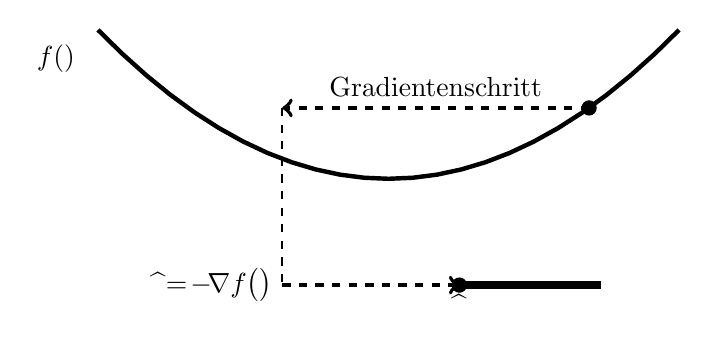
\begin{tikzpicture}[scale=0.9]
					\node [right] at (-5.1,1.7) {$f(\weights)$} ;
					\draw[ultra thick, domain=-4.1:4.1] plot (\x,  {(1/8)*\x*\x});
					\draw [fill] (2.83,1) circle [radius=0.1] node[right] {$\weights$};
					\draw[line width =0.5mm,dashed,->] (2.83,1) -- node[midway,above] {Gradientenschritt} (-1.5,1);
					\draw[line width =0.2mm,dashed] (-1.5,1) --(-1.5,-1.5)  node [below, left]{$\widehat{\weights}=\weights\!-\!\lrate \nabla f\big(\weights\big)$} ;
					\draw[line width =0.5mm,dashed,->] (-1.5,-1.5)  -- node[midway,above] {} (1,-1.5) ; 
					\draw [fill] (1,-1.5) circle [radius=0.1] node[below] {$\projection{\paramspace}{\widehat{\weights}}$};
					\draw[line width=1mm] (1,-1.5) -- (3,-1.5) node[midway, above] {$\paramspace$};
				\end{tikzpicture}
				\vspace*{-5mm}
			\end{center}
			\caption{Projizierter \gls{gd} erweitert einen einfachen \gls{gradstep} durch eine \gls{projection} zurück auf die zulässige Menge $\paramspace$.}
			\label{fig_projected_GD_dict}
		\end{figure}
	},
	first={projizierter Gradientenabstieg (projizierter GD)},
	text={projizierter GD}
}

\newglossaryentry{diffpriv}{
	name=differenzielle Privatsphäre (DP),
	description={
		Betrachten wir eine \gls{ml}-Methode $\algomap$, 
		die ein \gls{dataset} (z.\,B.\ das \gls{trainset} im Rahmen von \gls{erm}) einliest 
		und ein Ergebnis $\algomap(\dataset)$ liefert. Dieses Ergebnis kann entweder aus den 
		gelernten \gls{modelparams} oder den \gls{prediction}s für bestimmte \gls{datapoint}s bestehen. \\
		Die differenzielle \index{differenzielle Privatsphäre (DP)} Privatsphäre (DP) ist ein präzises Maß 
		für die \gls{privleakage}, die durch die Offenlegung dieses Ergebnisses entsteht. 
		Grob gesagt ist eine \gls{ml}-Methode dann differentielle privat, wenn sich die 
		\gls{probdist} des Ausgabewerts $\algomap(\dataset)$ nicht wesentlich ändert, 
		wenn das \gls{sensattr} eines einzelnen \gls{datapoint} im \gls{trainset} verändert wird. \\
		Wichtig ist, dass DP auf einem \gls{probmodel} der \gls{ml}-Methode basiert – 
		das heißt, wir interpretieren $\algomap(\dataset)$ als \gls{realization} einer \gls{rv}. 
		Die notwendige Zufälligkeit im Ergebnis kann durch gezieltes Hinzufügen einer 
		Realisierung einer zusätzlichen \gls{rv} (also durch das Hinzufügen von Rauschen) 
		erzeugt werden.
	},
	first = {differenzielle Privatsphäre (DP)},
	text={DP}
}

\newglossaryentry{stability}{
	name={Stabilität},
	description={
		Die \index{Stabilität} \textbf{Stabilität} ist eine wünschenswerte Eigenschaft einer \gls{ml}-Methode $\algomap$, 
		die ein \gls{dataset} $\dataset$ (z.\,B.\ ein \gls{trainset}) auf eine Ausgabe $\algomap(\dataset)$ abbildet. 
		Die Ausgabe $\algomap(\dataset)$ kann entweder aus den gelernten \gls{modelparams} oder aus 
		den \gls{prediction}s eines trainierten \gls{model} für einen bestimmten \gls{datapoint} bestehen. \\
		Intuitiv ist $\algomap$ stabil, wenn kleine Änderungen im Eingabe-\gls{dataset} $\dataset$ nur zu 
		kleinen Änderungen in der Ausgabe $\algomap(\dataset)$ führen. Es existieren mehrere formale 
		Begriffsbildungen von Stabilität, mit denen sich Schranken für den \gls{generalization}-Fehler oder das 
		\gls{risk} der Methode herleiten lassen (siehe \cite[Kap.~13]{ShalevMLBook}). \\
		Zur Veranschaulichung betrachte die drei in Abbildung~\ref{fig_three_data_stability} dargestellten \gls{dataset}s, 
		die unabhängig voneinander aus derselben \gls{data}-erzeugenden \gls{probdist} gezogen wurden. 
		Da die optimalen \gls{modelparams} durch diese zugrunde liegende \gls{probdist} bestimmt sind, 
		sollte eine genaue \gls{ml}-Methode $\algomap$ für alle drei \gls{dataset}s dieselbe (oder eine sehr ähnliche) 
		Ausgabe $\algomap(\dataset)$ liefern. Mit anderen Worten: Eine sinnvolle $\algomap$ muss robust 
		gegenüber der Variabilität in \gls{sample}-\gls{realization}en aus derselben \gls{probdist} sein – 
		d.\,h.\ sie muss stabil sein.
		\begin{figure}[H]
			\centering
			\begin{tikzpicture}
				\begin{axis}[
					axis lines=none,
					xlabel={$\sampleidx$},
					legend pos=north west,
					ymin=0, ymax=10,
					xtick={1,2,3,4,5},
					grid style=dashed,
					every axis plot/.append style={very thick}
					]
					% Dataset 1
					\addplot+[only marks,mark=*] coordinates {
						(1,2) (2,4) (3,3) (4,5) (5,7)
					};
					% Dataset 2
					\addplot+[only marks,mark=square*] coordinates {
						(1,3) (2,2) (3,6) (4,4) (5,5)
					};
					% Dataset 3
					\addplot+[only marks,mark=triangle*] coordinates {
						(1,5) (2,7) (3,4) (4,6) (5,3)
					};
				\end{axis}
			\end{tikzpicture}
			\caption{Drei \gls{dataset}s $\dataset^{(*)}$, $\dataset^{(\square)}$ und $\dataset^{(\triangle)}$, 
				die jeweils unabhängig aus derselben \gls{data}-erzeugenden \gls{probdist} gezogen wurden. 
				Eine stabile \gls{ml}-Methode sollte bei Training auf einem dieser \gls{dataset}s jeweils 
				ähnliche Ausgaben liefern. \label{fig_three_data_stability}}
		\end{figure}
	},
	first = {Stabilität},
	text = {Stabilität}
}

\newglossaryentry{privprot}{
	name={Privatsphärenschutz},
	description={
		\index{Privatsphärenschutz} Betrachte eine \gls{ml}-Methode $\algomap$, die ein \gls{dataset} $\dataset$ 
		als Eingabe erhält und eine Ausgabe $\algomap(\dataset)$ liefert. Die Ausgabe kann die gelernten 
		\gls{modelparams} $\widehat{\weights}$ oder die \gls{prediction} $\learnthypothesis(\featurevec)$ 
		für einen bestimmten \gls{datapoint} mit \gls{feature}n $\featurevec$ sein. \\
		Viele wichtige \gls{ml}-Anwendungen verarbeiten \gls{datapoint}s, die Menschen repräsentieren. 
		Jeder \gls{datapoint} ist charakterisiert durch \gls{feature}n $\featurevec$, eventuell ein \gls{label} $\truelabel$ 
		und ein \gls{sensattr} $\sensattr$ (z.\,B.\ eine kürzliche medizinische Diagnose). \\
		Grob gesagt bedeutet Privatsphärenschutz, dass es unmöglich sein sollte, aus der Ausgabe 
		$\algomap(\dataset)$ Rückschlüsse auf die \gls{sensattr}s einzelner \gls{datapoint}s in $\dataset$ zu ziehen. 
		Mathematisch verlangt Privatsphärenschutz, dass die Abbildung $\algomap(\dataset)$ nicht invertierbar ist. \\
		Im Allgemeinen reicht es jedoch nicht aus, $\algomap(\dataset)$ nur nicht invertierbar zu machen. 
		Vielmehr muss $\algomap(\dataset)$ hinreichend nicht invertierbar sein.
	},
	first = {Privatsphärenschutz},
	text = {Privatsphärenschutz}
}

\newglossaryentry{privleakage}{
	name={Privacy Leakage (Informationsleckage)},
	description={
		Betrachte eine \gls{ml}-Anwendung, die ein \gls{dataset} $\dataset$ verarbeitet und 
		eine Ausgabe liefert, z. B. \gls{prediction}en für neue \gls{datapoint}e. Privacy Leakage 
		entsteht, wenn die Ausgabe Informationen über eine private (oder sensible) \gls{feature} 
		eines \gls{datapoint}es (z. B. einer Person) aus $\dataset$ enthält. 
		Basierend auf einem \gls{probmodel} für die \gls{data}-Erzeugung kann man die Privacy Leakage 
		über die \gls{mutualinformation} zwischen der Ausgabe und dem sensiblen \gls{feature} messen. 
		Eine weitere quantitative Messgröße für Privacy Leakage ist die \gls{diffpriv}. 
		Die Zusammenhänge verschiedener Privacy-Maße wurden in der Literatur untersucht 
		(siehe \cite{InfThDiffPriv}).
	},
	first={Privacy Leakage (Informationsleckage)},
	text={Privacy Leakage}
}
